
\documentclass[landscape, DIV=99, 14pt]{scrartcl}

\renewcommand*{\familydefault}{\sfdefault}

\RequirePackage{graphicx}
\RequirePackage{hyperref}
\RequirePackage[gen]{eurosym}
\RequirePackage{multirow}
\RequirePackage{booktabs}
\RequirePackage[table]{xcolor}
\RequirePackage{siunitx}
\RequirePackage{etoolbox}
\RequirePackage{etoolbox}

\setlength{\parindent}{0cm}

\robustify\bfseries
\robustify\itshape

\begin{document}
\sisetup{detect-all = true}

\twocolumn
\section*{Zusammenfassung BMW Kosten}
\null
\vspace{1cm}
\begin{center}
%                           trim={<left> <lower> <right> <upper>}
\includegraphics[width=10cm, trim={4cm 0 4cm 5cm}]{images/kosten_verteilung.png}
\end{center}

\includegraphics[width=1.4\columnwidth]{images/kosten_maximus.png}

\pagebreak

\begin{itemize}
    \item Wertverlust
    \begin{itemize}
        \item Kaufpreis minus Verkaufspreis
    \end{itemize}
    \item Kraftstoffe
    \begin{itemize}
        \item Summe aller Tankstellenbesuche
    \end{itemize}
    \item Wartung und Reparatur
    \begin{itemize}
        \item Regul\"are Wartungsarbeiten (\"Olwechsel, etc)
        \item Reparaturen Aufgrund technischer Defekte
        \item Unfallsch\"aden
    \end{itemize}
    \item Versicherung
    \begin{itemize}
        \item J\"ahrlicher Versicherungsbeitrag
        \item Mobilit\"ats-Service
    \end{itemize}
    \item Steuern
    \begin{itemize}
            \item J\"ahrliche KFZ-Steuer
    \end{itemize}
\end{itemize}


\twocolumn

\section*{BMW 318d Kredit}
\begin{center}
\includegraphics[width=0.5\textheight]{images/bmw-318d-kredit-boundaries.png}
\null
\vspace{0.5cm}
\includegraphics[width=0.5\textheight]{images/bmw-318d-kredit-calc_df.png}
\end{center}

\pagebreak
\begin{center}
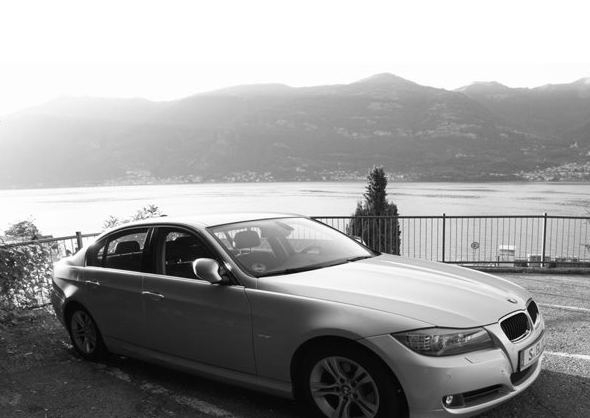
\includegraphics[width=0.9\columnwidth]{cars/bmw-3er-maximus.png}

BMW 318d Kredit
\end{center}

\begin{itemize}
    \item Baujahr: 2011 $\rightarrow$ Laufzeit: 7 Jahre
    \item \href{https://de.wikipedia.org/wiki/BMW_E90}{Weblink}
    \item \emph{Realer} Spritpreis \"uber Haltedauer: 1.19 \euro{}/l
    \item Antrieb: Diesel, mit 137 PS
    \item Restwert nach Faustformel (Neupreis $\times$ 20.5\%): 3472.26 \euro{}
\end{itemize}

\begin{small}
\emph{Meinung Nataliya:} 0/10: 
        
\emph{Meinung Grzegorz:} 7/10: Eigentlich ein super Auto: bequem, sportlich und langstreckentauglich. Aber zu wenig Platz und viel zu viele Reparaturen.
\end{small}

\pagebreak


\twocolumn

\section*{Nissan Micra Kredit}
\begin{center}
\includegraphics[width=0.5\textheight]{images/nissan-micra-kredit-boundaries.png}
\null
\vspace{0.5cm}
\includegraphics[width=0.5\textheight]{images/nissan-micra-kredit-calc_df.png}
\end{center}

\pagebreak
\begin{center}
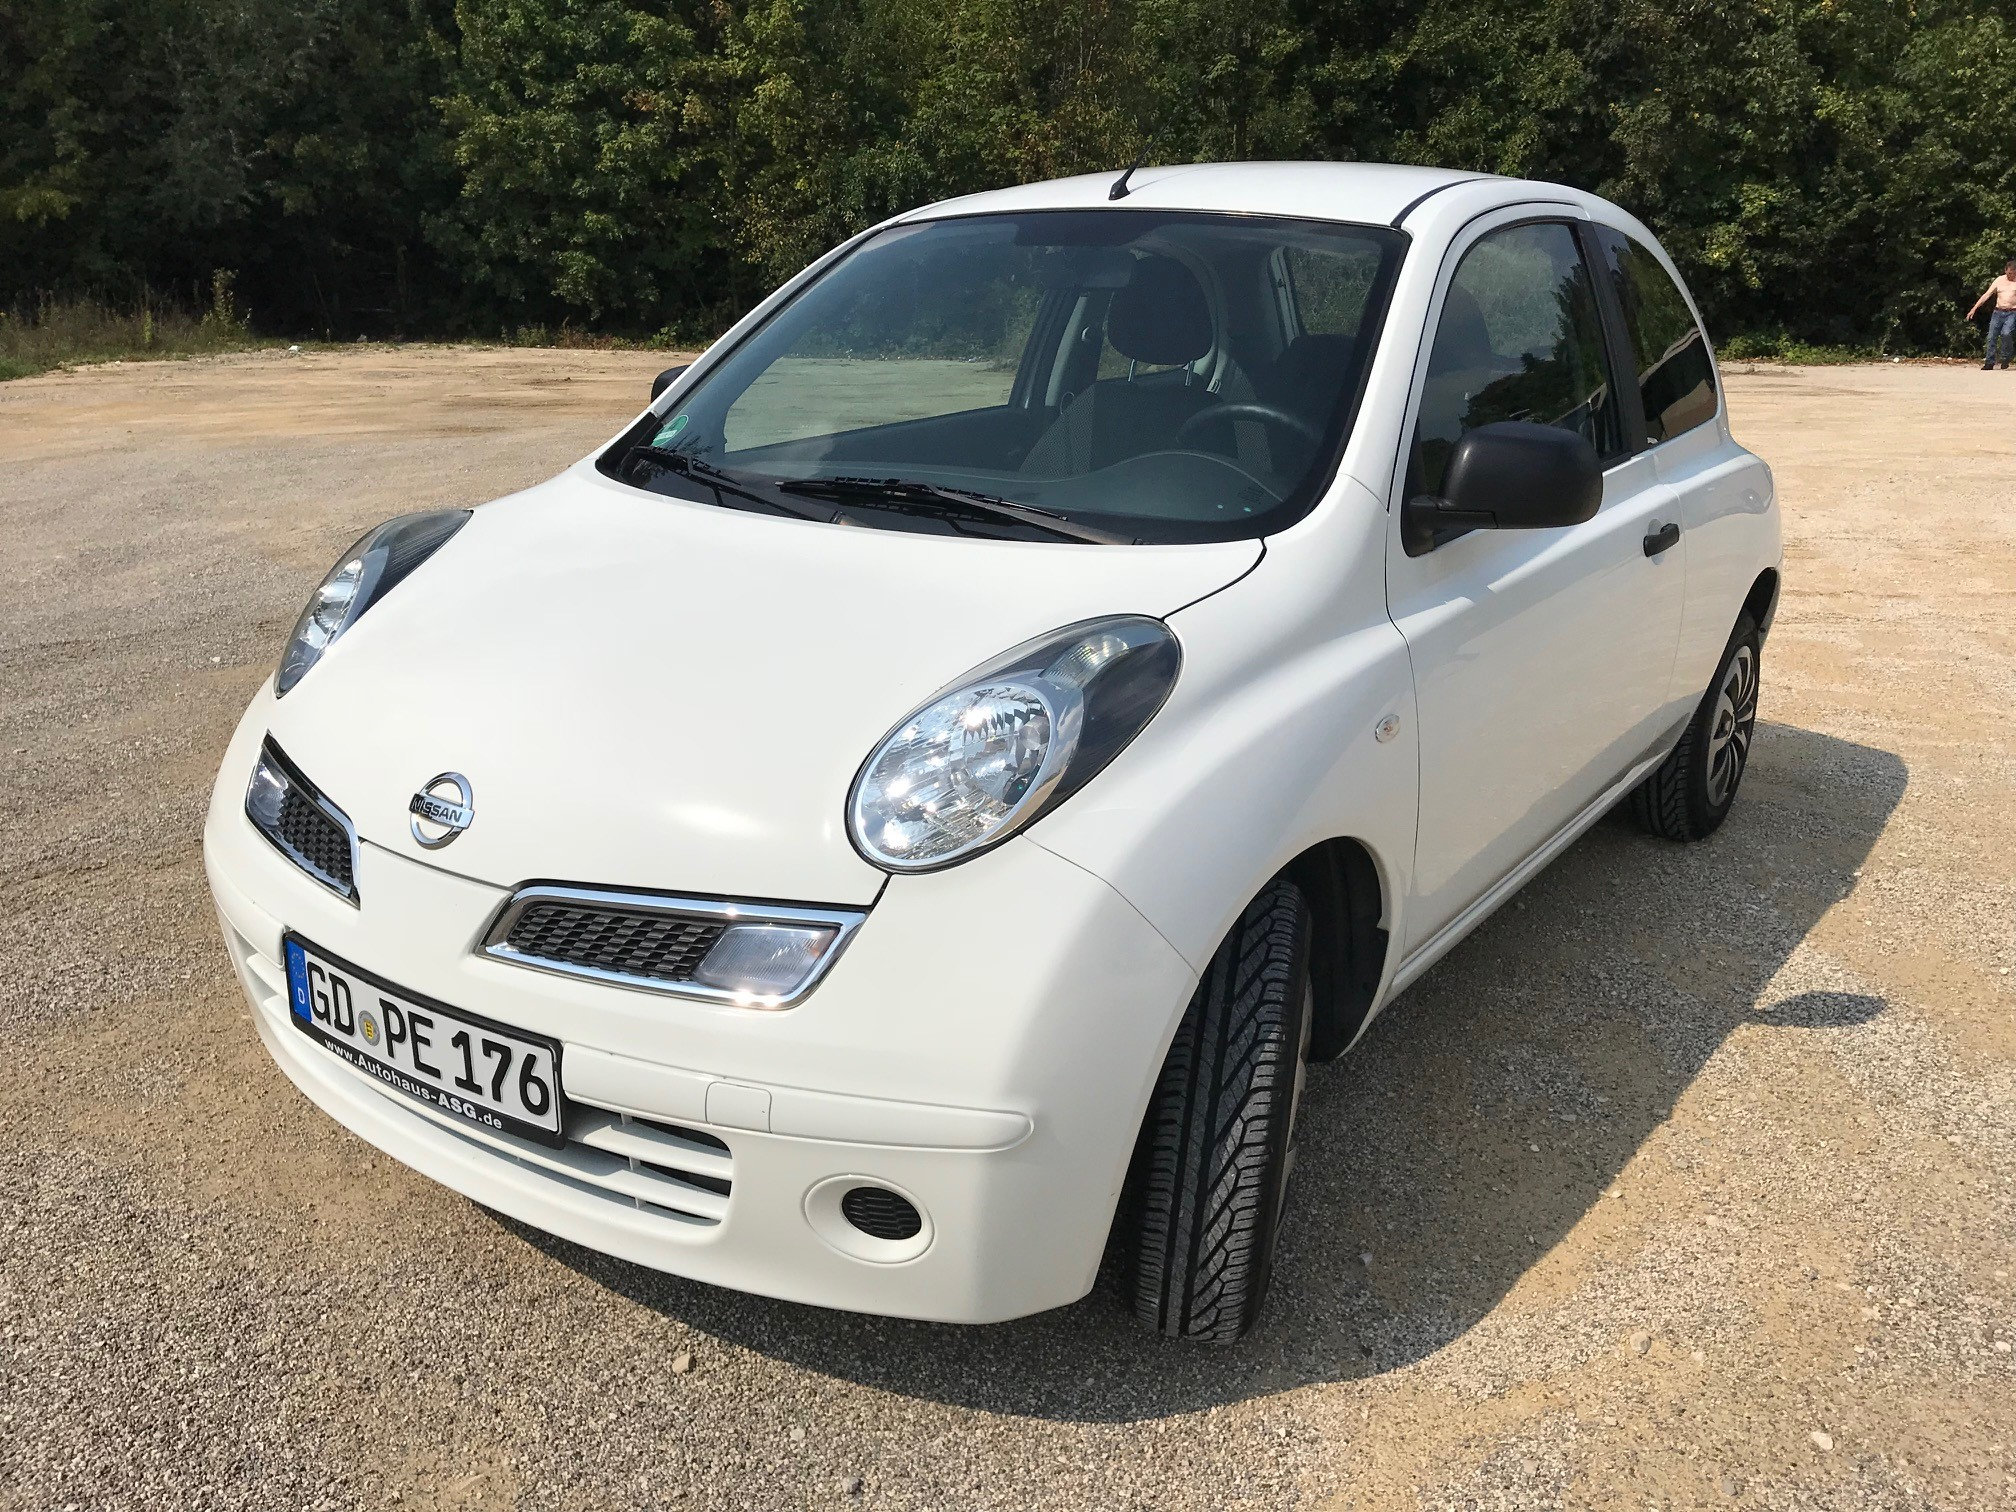
\includegraphics[width=0.9\columnwidth]{cars/nissan-micra.jpg}

Nissan Micra Kredit
\end{center}

\begin{itemize}
    \item Baujahr: 2011 $\rightarrow$ Laufzeit: 6 Jahre
    \item \href{https://de.wikipedia.org/wiki/Nissan_Micra\#Micra_(K12,_2003%E2%80%932010)}{Weblink}
    \item \emph{Realer} Spritpreis \"uber Haltedauer: 1.36 \euro{}/l
    \item Antrieb: Benzin, mit 65 PS
    \item Restwert nach Faustformel (Neupreis $\times$ 28.1\%): 926.03 \euro{}
\end{itemize}

\begin{small}
\emph{Meinung Nataliya:} 0/10: 
        
\emph{Meinung Grzegorz:} 6/10: Ein tolles Auto f\"ur den Preis. Sehr zuverl\"assig. Aber ein bisschen unbequem und extrem laut im Inneraum.
\end{small}

\pagebreak


\twocolumn

\section*{VW up! Leasing}
\begin{center}
\includegraphics[width=0.5\textheight]{images/vw-up-leasing-boundaries.png}
\null
\vspace{0.5cm}
\includegraphics[width=0.5\textheight]{images/vw-up-leasing-calc_df.png}
\end{center}

\pagebreak
\begin{center}
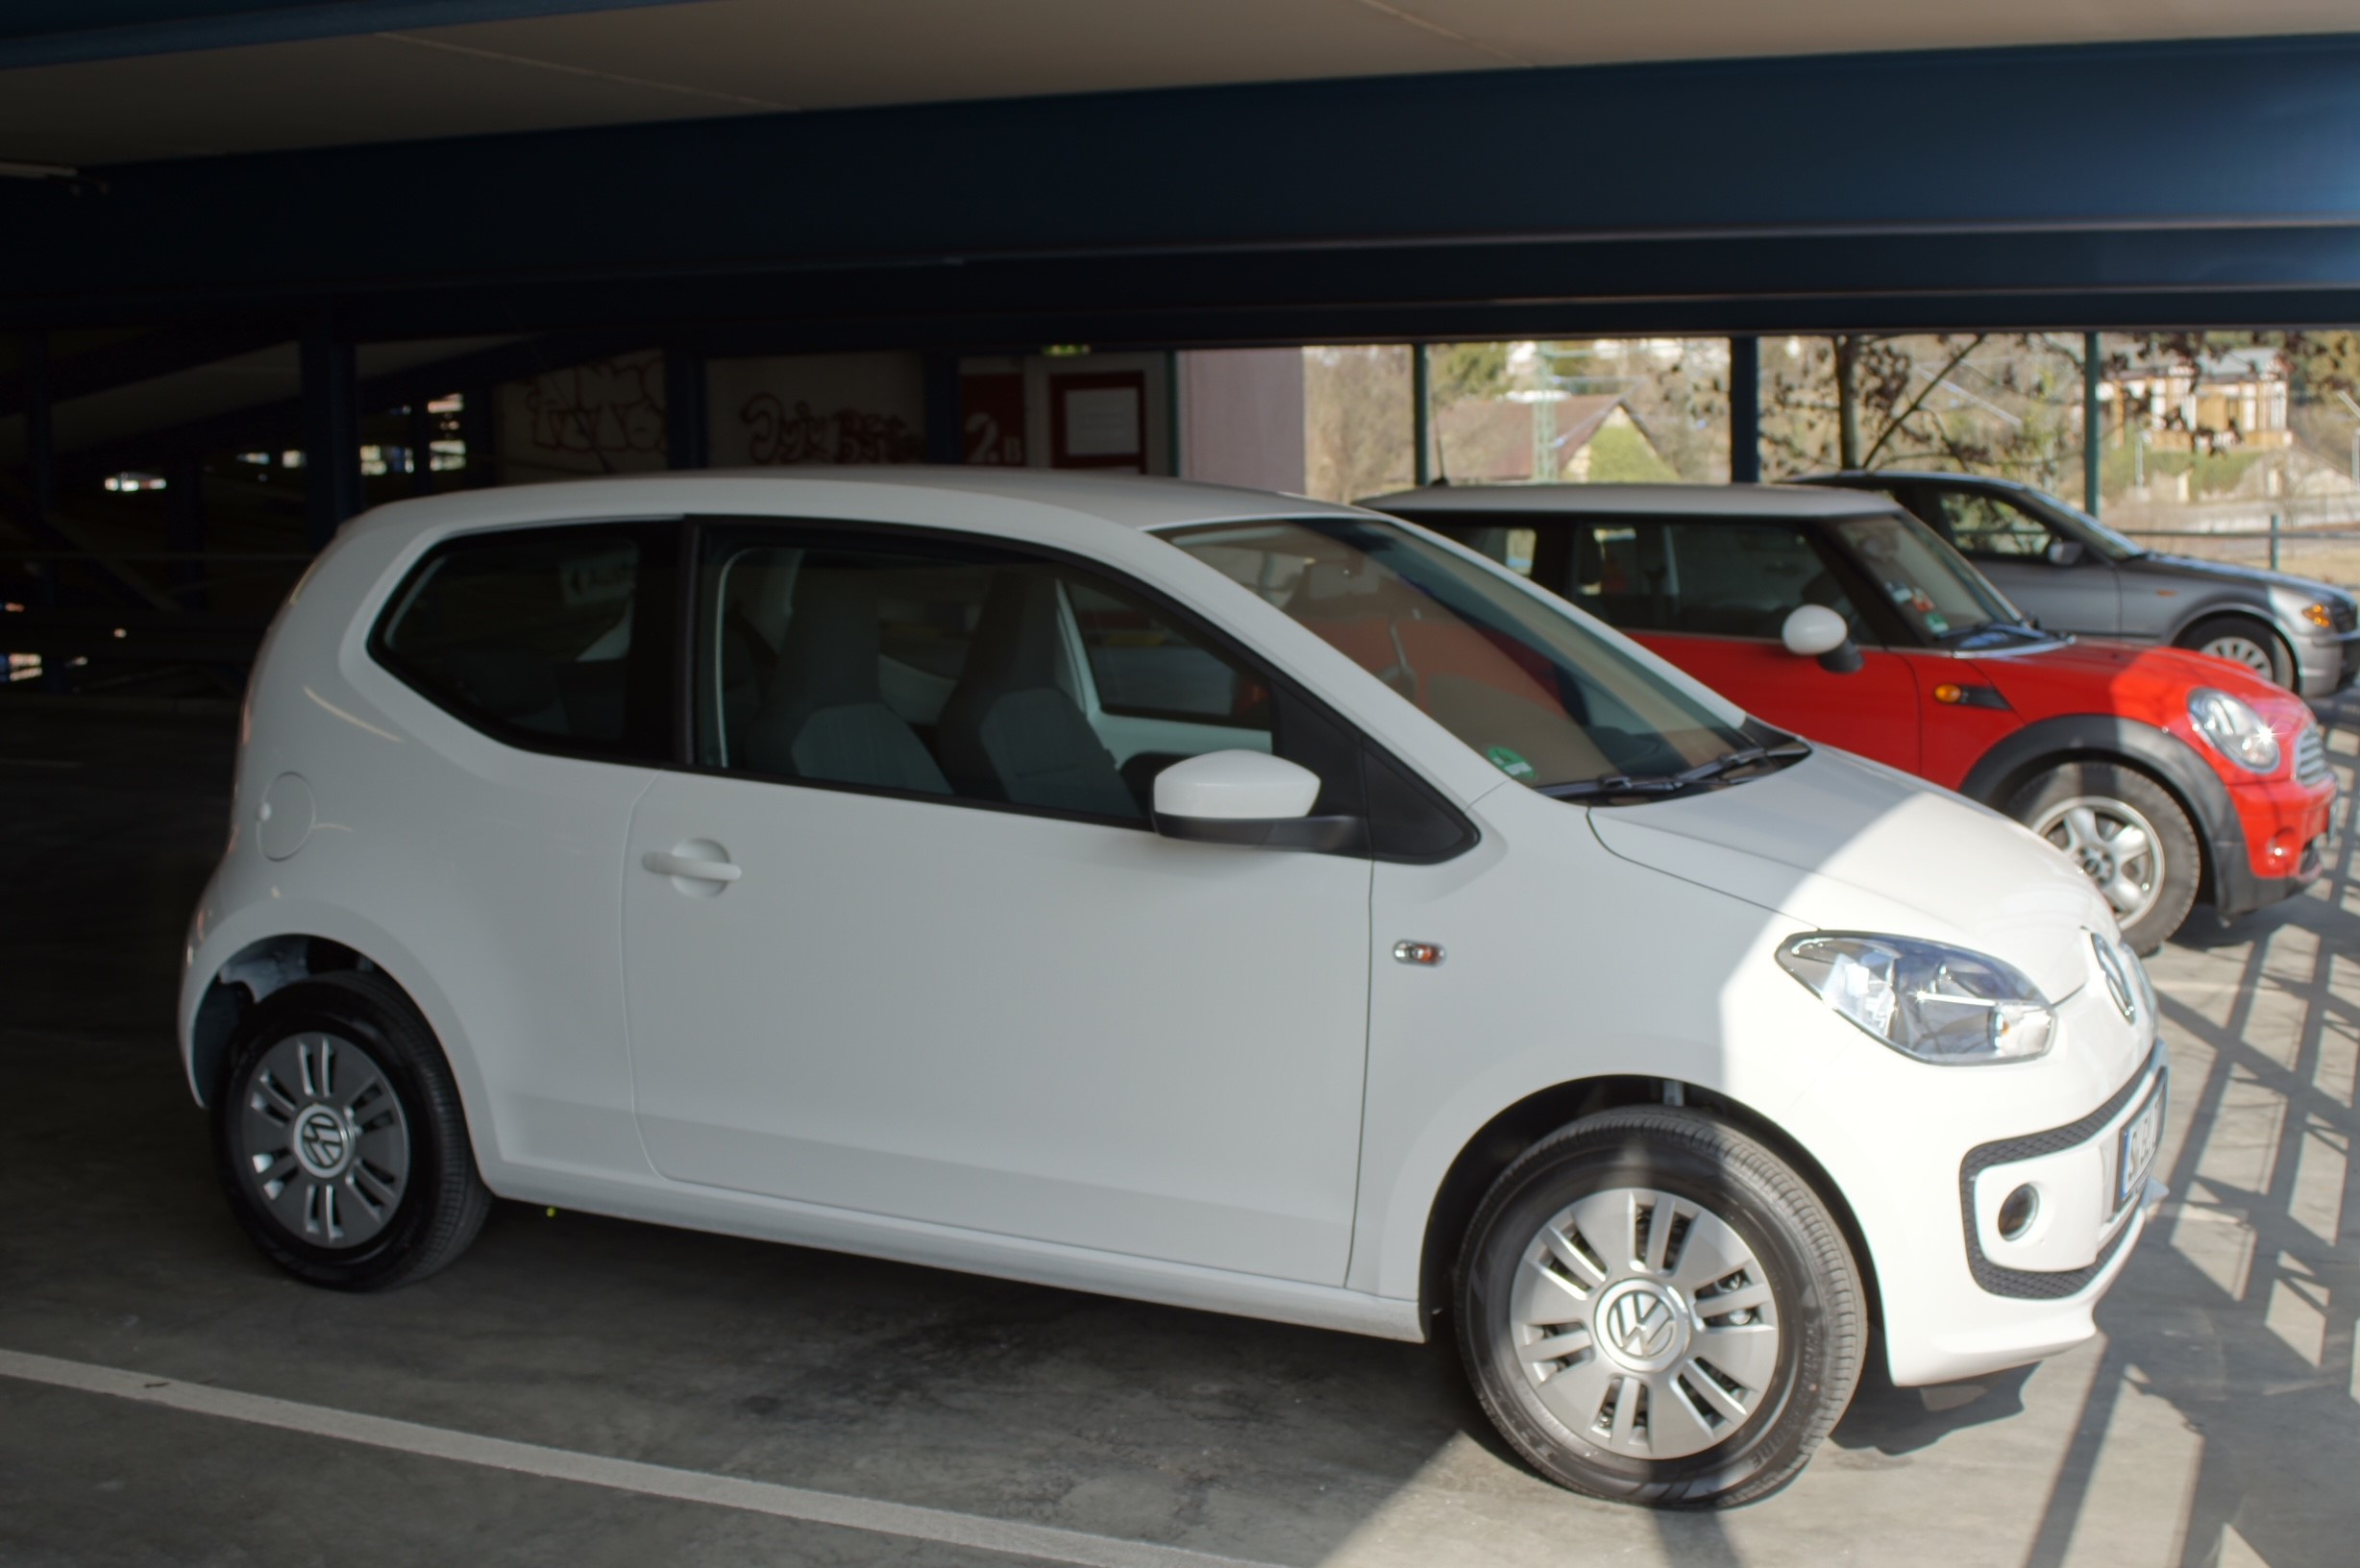
\includegraphics[width=0.9\columnwidth]{cars/vw-up.jpg}

VW up! Leasing
\end{center}

\begin{itemize}
    \item Baujahr: 2012 $\rightarrow$ Laufzeit: 3 Jahre
    \item \href{https://www.volkswagen.de/de/modelle/up.html}{Weblink}
    \item \emph{Realer} Spritpreis \"uber Haltedauer: 1.54 \euro{}/l
    \item Antrieb: Benzin, mit 60 PS
    \item Kein Restwert, da Leasingfahrzeug
\end{itemize}

\begin{small}
\emph{Meinung Nataliya:} 0/10: 
        
\emph{Meinung Grzegorz:} 5/10: Ich war sehr unzufrieden mit dem up. Er hat zwar ein gutes Fahrwerk und geringe Innenger\"ausche, aber ich fand den Verbrauch und die Wartungskosten viel zu hoch f\"ur so ein kleines Auto.
\end{small}

\pagebreak


\twocolumn

\section*{Tesla Model Y Kredit}
\begin{center}
\includegraphics[width=0.5\textheight]{images/tesla-model-y-kredit-boundaries.png}
\null
\vspace{0.5cm}
\includegraphics[width=0.5\textheight]{images/tesla-model-y-kredit-calc_df.png}
\end{center}

\pagebreak
\begin{center}
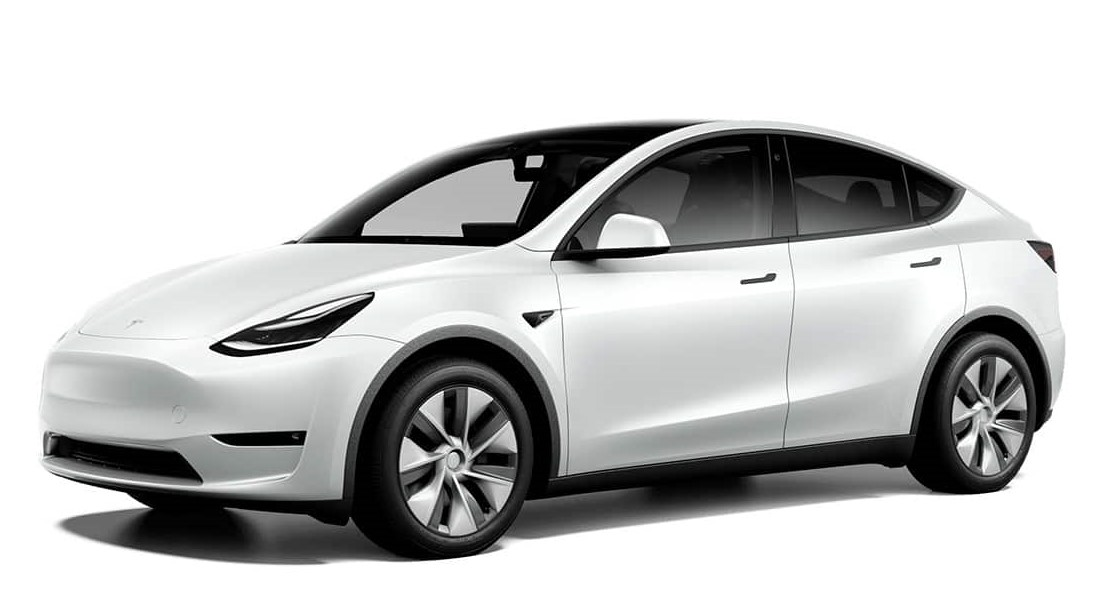
\includegraphics[width=0.9\columnwidth]{cars/tesla-model-y.jpg}

Tesla Model Y Kredit
\end{center}

\begin{itemize}
    \item Baujahr: 2022 $\rightarrow$ Laufzeit: 7 Jahre
    \item \href{https://www.tesla.com/de_de/modely/design\#overview}{Weblink}
    \item \emph{Gesch\"atzter} Spritpreis \"uber Haltedauer: 0.31 \euro{}/kWh
    \item Antrieb: Strom, mit 514 PS
    \item Restwert nach Faustformel (Neupreis $\times$ 19.8\%): 10510.58 \euro{}
\end{itemize}

\begin{small}
\emph{Meinung Nataliya:} 8/10: 
        
\emph{Meinung Grzegorz:} 8/10: Sehr bequemes, luxuri\"oses Auto. Viel Platz, viel Leistung, gro\ss{}e Reichweite. Schlechtes Kofferraum Management, Keine Hutablage, keine Sicherung unter dem Sitz.
\end{small}

\pagebreak


\twocolumn

\section*{Tesla Model Y Leasing}
\begin{center}
\includegraphics[width=0.5\textheight]{images/tesla-model-y-leasing-boundaries.png}
\null
\vspace{0.5cm}
\includegraphics[width=0.5\textheight]{images/tesla-model-y-leasing-calc_df.png}
\end{center}

\pagebreak
\begin{center}
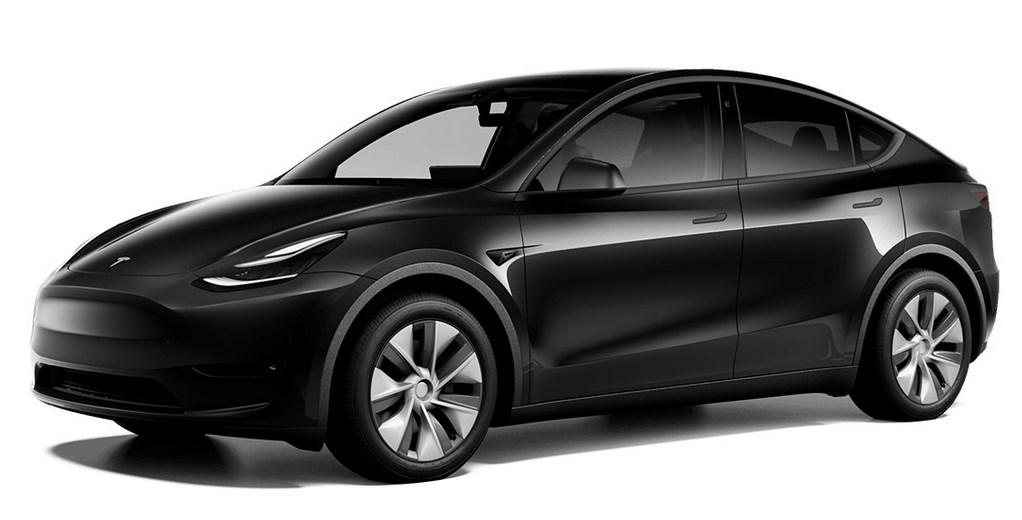
\includegraphics[width=0.9\columnwidth]{cars/tesla-model-y-leasing.jpg}

Tesla Model Y Leasing
\end{center}

\begin{itemize}
    \item Baujahr: 2022 $\rightarrow$ Laufzeit: 4 Jahre
    \item \href{https://www.tesla.com/de_de/modely/design\#overview}{Weblink}
    \item \emph{Gesch\"atzter} Spritpreis \"uber Haltedauer: 0.31 \euro{}/kWh
    \item Antrieb: Strom, mit 514 PS
    \item Kein Restwert, da Leasingfahrzeug
\end{itemize}

\begin{small}
\emph{Meinung Nataliya:} 8/10: 
        
\emph{Meinung Grzegorz:} 8/10: Sehr bequemes, luxuri\"oses Auto. Viel Platz, viel Leistung, gro\ss{}e Reichweite. Schlechtes Kofferraum Management, Keine Hutablage, keine Sicherung unter dem Sitz.
\end{small}

\pagebreak


\twocolumn

\section*{Tesla Model 3 Kredit}
\begin{center}
\includegraphics[width=0.5\textheight]{images/tesla-model-3-kredit-boundaries.png}
\null
\vspace{0.5cm}
\includegraphics[width=0.5\textheight]{images/tesla-model-3-kredit-calc_df.png}
\end{center}

\pagebreak
\begin{center}
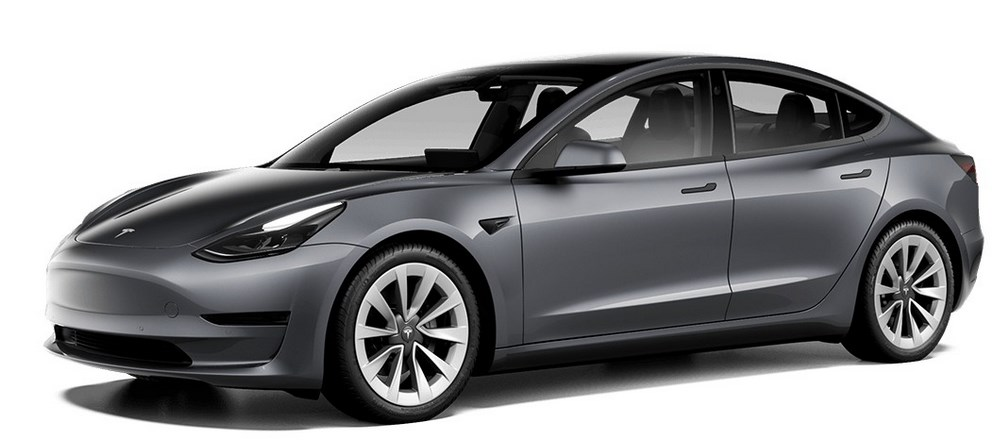
\includegraphics[width=0.9\columnwidth]{cars/tesla-model-3.jpg}

Tesla Model 3 Kredit
\end{center}

\begin{itemize}
    \item Baujahr: 2022 $\rightarrow$ Laufzeit: 7 Jahre
    \item \href{https://www.tesla.com/de_de/model3/design\#overview}{Weblink}
    \item \emph{Gesch\"atzter} Spritpreis \"uber Haltedauer: 0.31 \euro{}/kWh
    \item Antrieb: Strom, mit 325 PS
    \item Restwert nach Faustformel (Neupreis $\times$ 19.8\%): 8724.75 \euro{}
\end{itemize}

\begin{small}
\emph{Meinung Nataliya:} 0/10: 
        
\emph{Meinung Grzegorz:} 0/10: 
\end{small}

\pagebreak


\twocolumn

\section*{Tesla Model 3 Leasing}
\begin{center}
\includegraphics[width=0.5\textheight]{images/tesla-model-3-leasing-boundaries.png}
\null
\vspace{0.5cm}
\includegraphics[width=0.5\textheight]{images/tesla-model-3-leasing-calc_df.png}
\end{center}

\pagebreak
\begin{center}
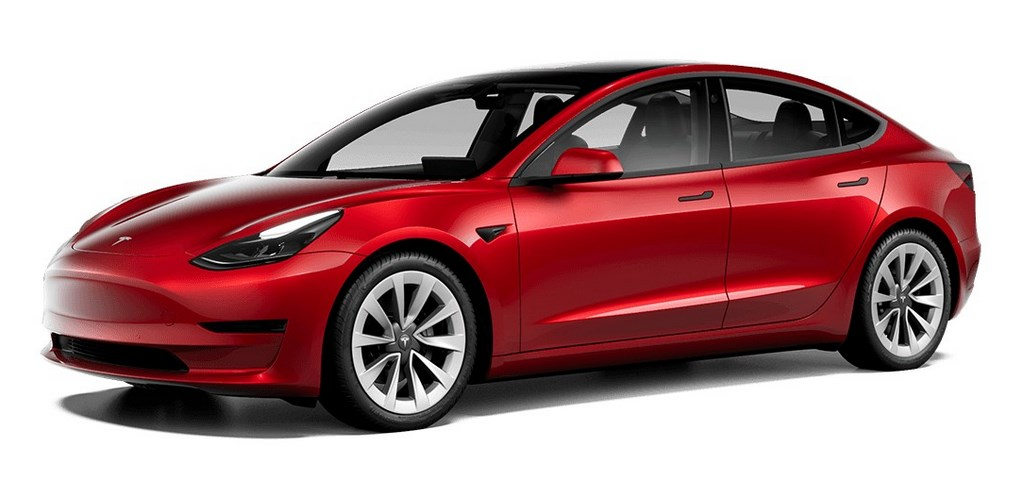
\includegraphics[width=0.9\columnwidth]{cars/tesla-model-3-leasing.jpg}

Tesla Model 3 Leasing
\end{center}

\begin{itemize}
    \item Baujahr: 2022 $\rightarrow$ Laufzeit: 4 Jahre
    \item \href{https://www.tesla.com/de_de/model3/design\#overview}{Weblink}
    \item \emph{Gesch\"atzter} Spritpreis \"uber Haltedauer: 0.31 \euro{}/kWh
    \item Antrieb: Strom, mit 325 PS
    \item Kein Restwert, da Leasingfahrzeug
\end{itemize}

\begin{small}
\emph{Meinung Nataliya:} 0/10: 
        
\emph{Meinung Grzegorz:} 0/10: 
\end{small}

\pagebreak


\twocolumn

\section*{Mazda 6 Kredit}
\begin{center}
\includegraphics[width=0.5\textheight]{images/mazda-6-kredit-boundaries.png}
\null
\vspace{0.5cm}
\includegraphics[width=0.5\textheight]{images/mazda-6-kredit-calc_df.png}
\end{center}

\pagebreak
\begin{center}
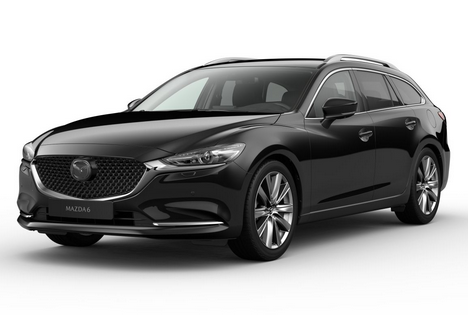
\includegraphics[width=0.9\columnwidth]{cars/mazda-6-neu.png}

Mazda 6 Kredit
\end{center}

\begin{itemize}
    \item Baujahr: 2022 $\rightarrow$ Laufzeit: 7 Jahre
    \item \href{https://konfigurator.meinauto.de/mazda/neuwagen/48-6/angebote/6-kombi/konfigurator/\#!/extras/exclusive-line/8846370/10,11/private/65352-5416-204698/984/61c9aa657e74c/cash-purchase/32545--287374/48,0,10000,0,0,0,0,0,}{Weblink}
    \item \emph{Gesch\"atzter} Spritpreis \"uber Haltedauer: 1.70 \euro{}/l
    \item Antrieb: Benzin, mit 192 PS
    \item Restwert nach Faustformel (Neupreis $\times$ 19.8\%): 6080.38 \euro{}
\end{itemize}

\begin{small}
\emph{Meinung Nataliya:} 6/10: 
        
\emph{Meinung Grzegorz:} 4/10: Tolles Au\ss{}endesign, sehr sch\"oner Innenraum und gro\ss{}er Kofferaum. Motor schwach und klapprig, Innenger\"ausche laut, Sitze ohne Seitenhalt, viel Windger\"ausche, krasser Abgasgeruch im Inneraum. Hatten nach der Probefahrt Kopfschmerzen. Verbrauch leider am Ende nicht gepr\"uft, aber war w\"ahrend der Probefahrt oft Richtung 10 l/100km
\end{small}

\pagebreak


\twocolumn

\section*{Mazda 6 Leasing}
\begin{center}
\includegraphics[width=0.5\textheight]{images/mazda-6-leasing-boundaries.png}
\null
\vspace{0.5cm}
\includegraphics[width=0.5\textheight]{images/mazda-6-leasing-calc_df.png}
\end{center}

\pagebreak
\begin{center}
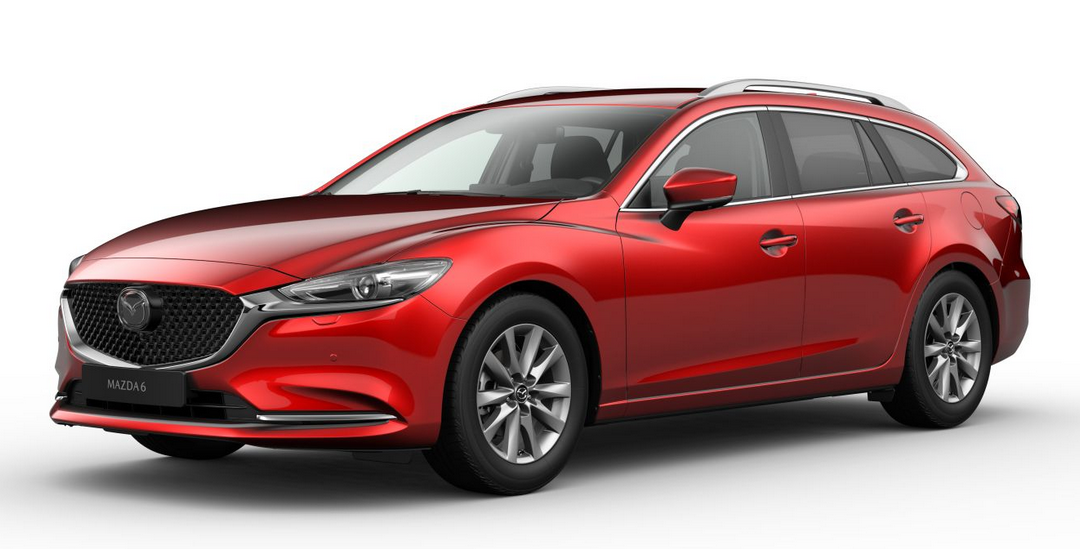
\includegraphics[width=0.9\columnwidth]{cars/mazda-6-leasing.png}

Mazda 6 Leasing
\end{center}

\begin{itemize}
    \item Baujahr: 2022 $\rightarrow$ Laufzeit: 3 Jahre
    \item \href{https://konfigurator.meinauto.de/mazda/neuwagen/48-6/angebote/6-kombi/konfigurator/\#!/extras/exclusive-line/8846370/10,11,15/private/65352-5416-204698/984/61c9aa657e74c/leasing/16040--249432/36,3000,15000,0,0,0,0,0,}{Weblink}
    \item \emph{Gesch\"atzter} Spritpreis \"uber Haltedauer: 1.70 \euro{}/l
    \item Antrieb: Benzin, mit 192 PS
    \item Kein Restwert, da Leasingfahrzeug
\end{itemize}

\begin{small}
\emph{Meinung Nataliya:} 6/10: 
        
\emph{Meinung Grzegorz:} 4/10: Tolles Au\ss{}endesign, sehr sch\"oner Innenraum und gro\ss{}er Kofferaum. Motor schwach und klapprig, Innenger\"ausche laut, Sitze ohne Seitenhalt, viel Windger\"ausche, krasser Abgasgeruch im Inneraum. Hatten nach der Probefahrt Kopfschmerzen. Verbrauch leider am Ende nicht gepr\"uft, aber war w\"ahrend der Probefahrt oft Richtung 10 l/100km
\end{small}

\pagebreak


\twocolumn

\section*{Hyundai Ioniq 5 Kredit}
\begin{center}
\includegraphics[width=0.5\textheight]{images/hyundai-ioniq-5-kredit-boundaries.png}
\null
\vspace{0.5cm}
\includegraphics[width=0.5\textheight]{images/hyundai-ioniq-5-kredit-calc_df.png}
\end{center}

\pagebreak
\begin{center}
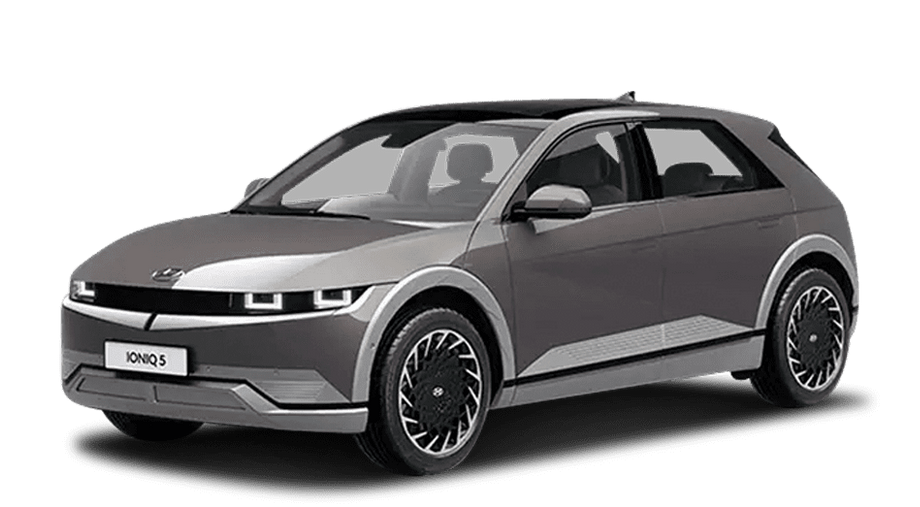
\includegraphics[width=0.9\columnwidth]{cars/hyundai-ioniq-5.png}

Hyundai Ioniq 5 Kredit
\end{center}

\begin{itemize}
    \item Baujahr: 2022 $\rightarrow$ Laufzeit: 7 Jahre
    \item \href{https://konfigurator.meinauto.de/hyundai/neuwagen/ioniq/angebote/ioniq-5/konfigurator/\#!/extras/-/8865700/14,19,41/private/104690-6897-293274/4864/61e90b0c48e55/cash-purchase/104690-6897-293274/24,9000,15000,0,0,0,0,0,}{Weblink}
    \item \emph{Gesch\"atzter} Spritpreis \"uber Haltedauer: 0.31 \euro{}/kWh
    \item Antrieb: Strom, mit 231 PS
    \item Restwert nach Faustformel (Neupreis $\times$ 19.8\%): 9630.77 \euro{}
\end{itemize}

\begin{small}
\emph{Meinung Nataliya:} 0/10: 
        
\emph{Meinung Grzegorz:} 0/10: Auf die Schnelle im Autosalon keinen gute Sitzposition gefunden. Kofferaum \"uberraschend klein f\"ur die Gr\"o\ss{}e. Verbrauch soll sehr hoch sein.
\end{small}

\pagebreak


\twocolumn

\section*{Hyundai Ioniq 5 Leasing}
\begin{center}
\includegraphics[width=0.5\textheight]{images/hyundai-ioniq-5-leasing-boundaries.png}
\null
\vspace{0.5cm}
\includegraphics[width=0.5\textheight]{images/hyundai-ioniq-5-leasing-calc_df.png}
\end{center}

\pagebreak
\begin{center}
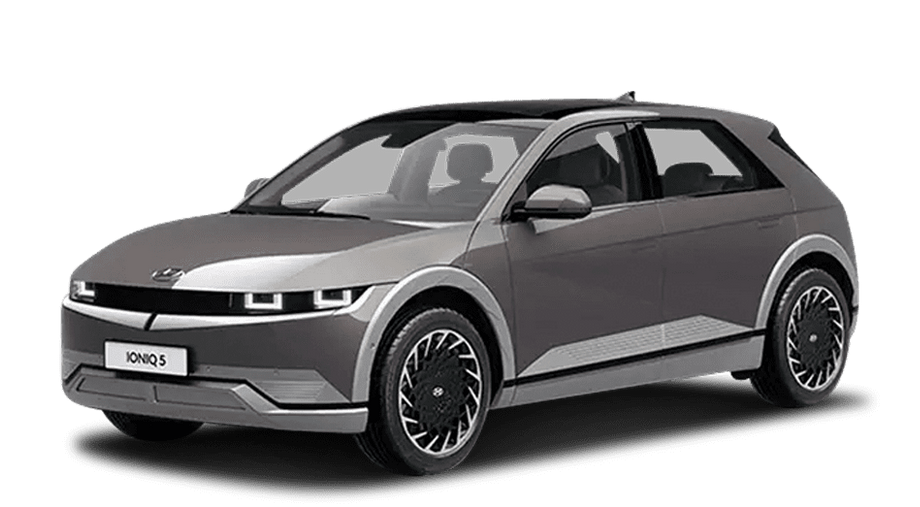
\includegraphics[width=0.9\columnwidth]{cars/hyundai-ioniq-5.png}

Hyundai Ioniq 5 Leasing
\end{center}

\begin{itemize}
    \item Baujahr: 2022 $\rightarrow$ Laufzeit: 2 Jahre
    \item \href{https://konfigurator.meinauto.de/hyundai/neuwagen/ioniq/angebote/ioniq-5/konfigurator/\#!/extras/-/8865700/14,19,41/private/104690-6897-293274/4864/61e90b0c48e55/leasing/104690-6897-293274/24,9000,15000,0,0,0,0,0,}{Weblink}
    \item \emph{Gesch\"atzter} Spritpreis \"uber Haltedauer: 0.31 \euro{}/kWh
    \item Antrieb: Strom, mit 231 PS
    \item Kein Restwert, da Leasingfahrzeug
\end{itemize}

\begin{small}
\emph{Meinung Nataliya:} 0/10: 
        
\emph{Meinung Grzegorz:} 0/10: Auf die Schnelle im Autosalon keinen gute Sitzposition gefunden. Kofferaum \"uberraschend klein f\"ur die Gr\"o\ss{}e. Verbrauch soll sehr hoch sein.
\end{small}

\pagebreak


\twocolumn

\section*{Kia ceed Kredit}
\begin{center}
\includegraphics[width=0.5\textheight]{images/kia-ceed-kredit-boundaries.png}
\null
\vspace{0.5cm}
\includegraphics[width=0.5\textheight]{images/kia-ceed-kredit-calc_df.png}
\end{center}

\pagebreak
\begin{center}
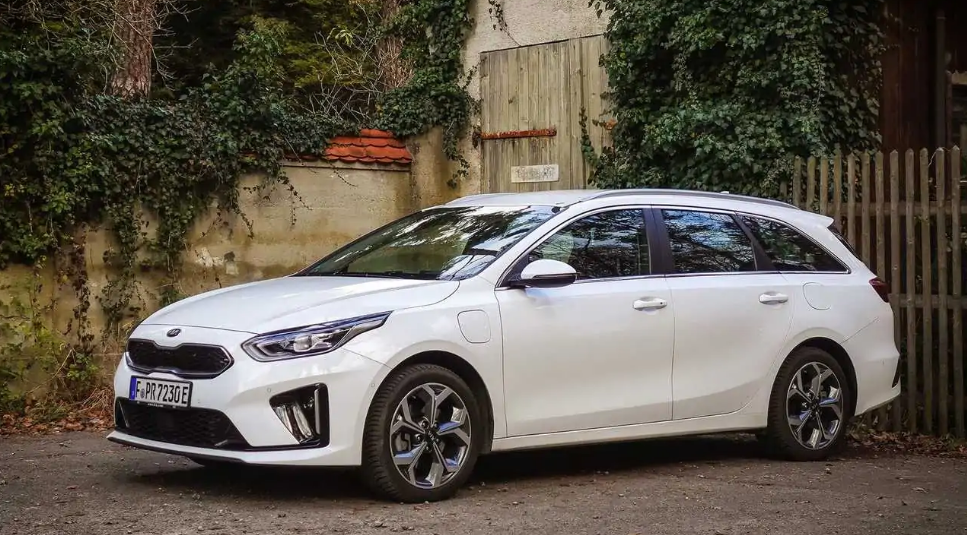
\includegraphics[width=0.9\columnwidth]{cars/kia-ceed-sportswagon.png}

Kia ceed Kredit
\end{center}

\begin{itemize}
    \item Baujahr: 2022 $\rightarrow$ Laufzeit: 7 Jahre
    \item \href{https://konfigurator.meinauto.de/kia/neuwagen/cee-d/angebote/cee-d-sporty-wagon/konfigurator/\#!/extras/spirit/8865371/3,11,27/private/109347-4167-291321/1321/61d21ce73c5db/cash-purchase/109348-8088-291322/48,0,10000,0,0,0,0,0,}{Weblink}
    \item \emph{Gesch\"atzter} Spritpreis \"uber Haltedauer: 1.70 \euro{}/l
    \item Antrieb: Benzin, mit 160 PS
    \item Restwert nach Faustformel (Neupreis $\times$ 19.8\%): 5002.18 \euro{}
\end{itemize}

\begin{small}
\emph{Meinung Nataliya:} 0/10: 
        
\emph{Meinung Grzegorz:} 0/10: 
\end{small}

\pagebreak


\twocolumn

\section*{Kia ceed Leasing}
\begin{center}
\includegraphics[width=0.5\textheight]{images/kia-ceed-leasing-boundaries.png}
\null
\vspace{0.5cm}
\includegraphics[width=0.5\textheight]{images/kia-ceed-leasing-calc_df.png}
\end{center}

\pagebreak
\begin{center}
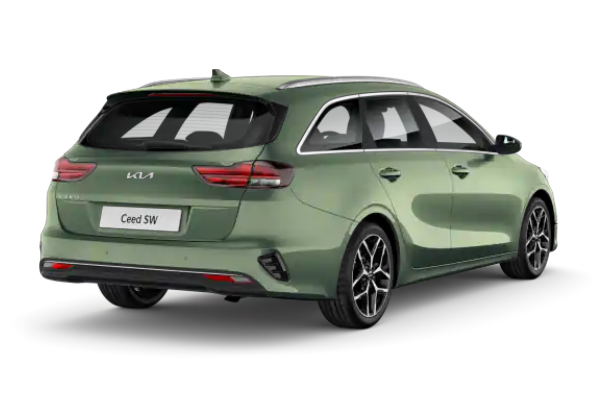
\includegraphics[width=0.9\columnwidth]{cars/kia-ceed-sportswagon-leasing.png}

Kia ceed Leasing
\end{center}

\begin{itemize}
    \item Baujahr: 2022 $\rightarrow$ Laufzeit: 3 Jahre
    \item \href{https://konfigurator.meinauto.de/kia/neuwagen/cee-d/angebote/cee-d-sporty-wagon/konfigurator/\#!/extras/spirit/8865371/3,11,27/private/109347-4167-291321/1321/61d21ce73c5db/leasing/109348-8088-291322/36,3000,15000,0,0,0,0,0,}{Weblink}
    \item \emph{Gesch\"atzter} Spritpreis \"uber Haltedauer: 1.70 \euro{}/l
    \item Antrieb: Benzin, mit 160 PS
    \item Kein Restwert, da Leasingfahrzeug
\end{itemize}

\begin{small}
\emph{Meinung Nataliya:} 0/10: 
        
\emph{Meinung Grzegorz:} 0/10: 
\end{small}

\pagebreak


\twocolumn

\section*{VW Passat Kredit}
\begin{center}
\includegraphics[width=0.5\textheight]{images/vw-passat-kredit-boundaries.png}
\null
\vspace{0.5cm}
\includegraphics[width=0.5\textheight]{images/vw-passat-kredit-calc_df.png}
\end{center}

\pagebreak
\begin{center}
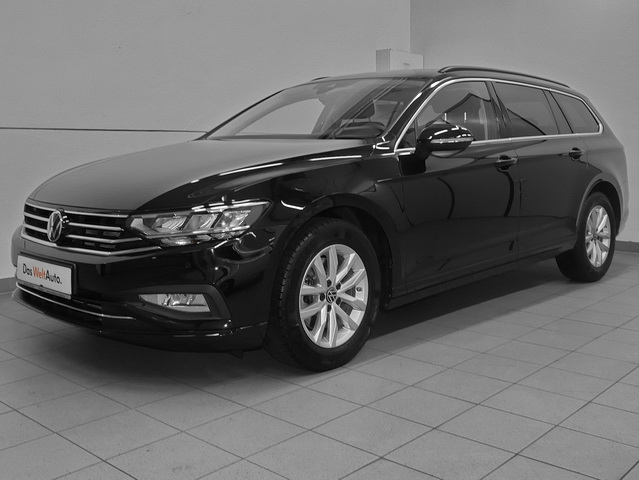
\includegraphics[width=0.9\columnwidth]{cars/vw-passat.jpg}

VW Passat Kredit
\end{center}

\begin{itemize}
    \item Baujahr: 2021 $\rightarrow$ Laufzeit: 7 Jahre
    \item \href{https://www.autosuche.de/auto/REVVNDQ3NjgwMjc5NzI=?t_manuf=BQ&t_petr=B&t_model=BQBM&t_gear=A&t_ez_fr=2020&t_pe_fr=35000&sort=PRICE_SALE&sortdirection=ASC&viewMode=tile}{Weblink}
    \item \emph{Gesch\"atzter} Spritpreis \"uber Haltedauer: 1.70 \euro{}/l
    \item Antrieb: Benzin, mit 150 PS
    \item Restwert nach Faustformel (Neupreis $\times$ 19.8\%): 5998.39 \euro{}
\end{itemize}

\begin{small}
\emph{Meinung Nataliya:} 0/10: 
        
\emph{Meinung Grzegorz:} 0/10: 
\end{small}

\pagebreak


\twocolumn

\section*{VW Passat Leasing}
\begin{center}
\includegraphics[width=0.5\textheight]{images/vw-passat-leasing-boundaries.png}
\null
\vspace{0.5cm}
\includegraphics[width=0.5\textheight]{images/vw-passat-leasing-calc_df.png}
\end{center}

\pagebreak
\begin{center}
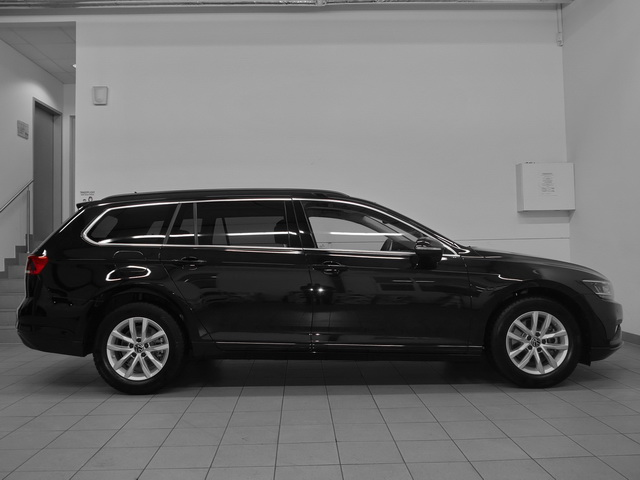
\includegraphics[width=0.9\columnwidth]{cars/vw-passat-leasing.jpg}

VW Passat Leasing
\end{center}

\begin{itemize}
    \item Baujahr: 2021 $\rightarrow$ Laufzeit: 3 Jahre
    \item \href{https://www.autosuche.de/auto/REVVNDQ3NjgwMjc5NzI=?t_manuf=BQ&t_petr=B&t_model=BQBM&t_gear=A&t_ez_fr=2020&t_pe_fr=35000&sort=PRICE_SALE&sortdirection=ASC&viewMode=tile}{Weblink}
    \item \emph{Gesch\"atzter} Spritpreis \"uber Haltedauer: 1.70 \euro{}/l
    \item Antrieb: Benzin, mit 150 PS
    \item Kein Restwert, da Leasingfahrzeug
\end{itemize}

\begin{small}
\emph{Meinung Nataliya:} 0/10: 
        
\emph{Meinung Grzegorz:} 0/10: 
\end{small}

\pagebreak


\twocolumn

\section*{Mercedes C 200 Kredit}
\begin{center}
\includegraphics[width=0.5\textheight]{images/mercedes-c-200-kredit-boundaries.png}
\null
\vspace{0.5cm}
\includegraphics[width=0.5\textheight]{images/mercedes-c-200-kredit-calc_df.png}
\end{center}

\pagebreak
\begin{center}
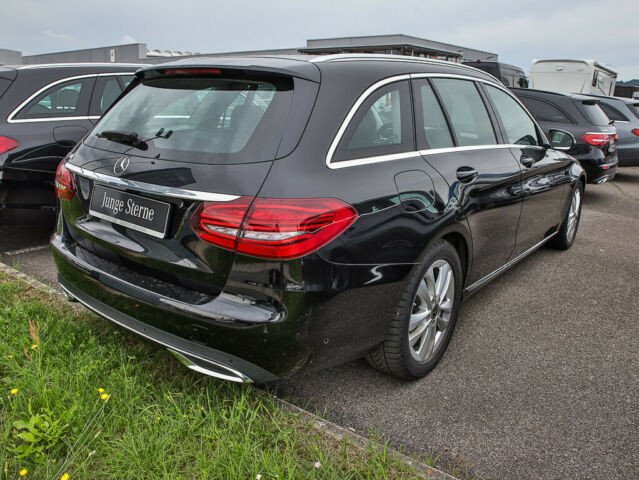
\includegraphics[width=0.9\columnwidth]{cars/mercedes-c-200-t-leasing.png}

Mercedes C 200 Kredit
\end{center}

\begin{itemize}
    \item Baujahr: 2019 $\rightarrow$ Laufzeit: 4 Jahre
    \item \href{https://suchen.mobile.de/fahrzeuge/details.html?action=parkItem&id=327113608}{Weblink}
    \item \emph{Gesch\"atzter} Spritpreis \"uber Haltedauer: 1.70 \euro{}/l
    \item Antrieb: Benzin, mit 184 PS
    \item Restwert nach Faustformel (Neupreis $\times$ 39.7\%): 10988.78 \euro{}
\end{itemize}

\begin{small}
\emph{Meinung Nataliya:} 0/10: 
        
\emph{Meinung Grzegorz:} 0/10: 
\end{small}

\pagebreak


\twocolumn

\section*{BMW GranT neu Kredit}
\begin{center}
\includegraphics[width=0.5\textheight]{images/bmw-grant-neu-kredit-boundaries.png}
\null
\vspace{0.5cm}
\includegraphics[width=0.5\textheight]{images/bmw-grant-neu-kredit-calc_df.png}
\end{center}

\pagebreak
\begin{center}
\includegraphics[width=0.9\columnwidth]{cars/bmw-gran-tourer-mulfinger.png}

BMW GranT neu Kredit
\end{center}

\begin{itemize}
    \item Baujahr: 2022 $\rightarrow$ Laufzeit: 7 Jahre
    \item \href{https://mulfinger.de/de/fahrzeugangebot/BMW/220i-GranTourer-Sport-DKG-HUD-LED-ParkAssNavi/page1/details-p5clkem9?manufacturer=5&model=2534&view=list}{Weblink}
    \item \emph{Gesch\"atzter} Spritpreis \"uber Haltedauer: 1.70 \euro{}/l
    \item Antrieb: Benzin, mit 192 PS
    \item Restwert nach Faustformel (Neupreis $\times$ 19.8\%): 8333.86 \euro{}
\end{itemize}

\begin{small}
\emph{Meinung Nataliya:} 0/10: 
        
\emph{Meinung Grzegorz:} 0/10: 
\end{small}

\pagebreak


\twocolumn

\section*{BMW GranT geb. Kredit}
\begin{center}
\includegraphics[width=0.5\textheight]{images/bmw-grant-geb-kredit-boundaries.png}
\null
\vspace{0.5cm}
\includegraphics[width=0.5\textheight]{images/bmw-grant-geb-kredit-calc_df.png}
\end{center}

\pagebreak
\begin{center}
\includegraphics[width=0.9\columnwidth]{cars/bmw-gran-tourer-mulfinger.png}

BMW GranT geb. Kredit
\end{center}

\begin{itemize}
    \item Baujahr: 2019 $\rightarrow$ Laufzeit: 7 Jahre
    \item \href{https://mulfinger.de/de/fahrzeugangebot/BMW/220i-GranTourer-Sport-DKG-HUD-LED-ParkAssNavi/page1/details-p5clkem9?manufacturer=5&model=2534&view=list}{Weblink}
    \item \emph{Gesch\"atzter} Spritpreis \"uber Haltedauer: 1.70 \euro{}/l
    \item Antrieb: Benzin, mit 192 PS
    \item Restwert nach Faustformel (Neupreis $\times$ 19.8\%): 4938.80 \euro{}
\end{itemize}

\begin{small}
\emph{Meinung Nataliya:} 0/10: 
        
\emph{Meinung Grzegorz:} 0/10: 
\end{small}

\pagebreak



\pagebreak

\onecolumn
\begin{figure}
\centering
Vergleich der monatlichen Kosten bei \euro{} 15000.00 Anzahlung bei Kreditfinanzierung und \euro{} 3000.00 bei Leasing.

Gesch\"atzer Kraftstoffpreis 1.70 \euro{}/l Benzin, bzw. 0.31 \euro{}/kWh


\includegraphics[width=0.95\columnwidth]{images/overview1.png}
\end{figure}
\vfill 



\end{document}
